\documentclass[long, final]{jobim2017}
% Available options are:
% - showframe 
% - draft
% - final [default]

\usepackage[utf8]{inputenc}

% WARNING: already loaded packages:
% - hyperref
% - times
% - color
% - xspace
% - graphicx
% - fancyhdr
% - fancybox
% - indentfirst
% - geometry
% - babel (options english,francais) :
%   choose the language with \selectlanguage{<language>}


\pagestyle{empty}
\addtolength{\parskip}{0.4\baselineskip}

%% Title of the paper (required)
\title{Data updates on Norine, the reference Non-Ribosomal Peptide knowledge base}

%% List of authors (separated by the macro \and).
%% Authors can be followed by \inst{<n>} macro.
%% The <n> parameter of the \inst macro should correspond to the <n>th institution
%% (see macro \institute below).
\author{Yoann \textsc{Dufresne}\inst{1} \and FirstName \textsc{LastName2}\inst{2} \and FirstName \textsc{LastName3}\inst{2}}

%% List of institutions (separated by the macro \and).
\institute{
 Équipe Bonsai, CRIStAL, université de Lille, INRIA Lille Nord Europe, Batiment M3, avenue Carl Gauss, 59655, Villeneuve d'Ascq, France
 \and
 Laboratory, Address, zip code, Town, Country 
}

% email of the corresponding author
\corresponding{yoann.dufresne0@gmail.com}





%% Abstract of the paper (required).
\abstract{%
 The abstract of the paper (optional for short contributions) must be typeset
 in italic, with \emph{Times New Roman} 11-point font. The left and right margins
 must be set to 3cm. \textcolor{red}{350 words maximum.}
}




%% List of keywords of the paper (required).
\keywords{Norine database, Non-Ribosomal Peptides, Update, Data curation}

\begin{document}

 % Si vous écrivez en français, commentez la ligne suivante
\selectlanguage{english}
 % Si vous écrivez en francais, décommentez la ligne suivante...
 % \selectlanguage{francais}

   \maketitle





\section{Introduction}

Norine, first released in 2006[TODO], remains the unique platform dedicated to computational biology analysis of non-ribosomal peptides (NRPs). The NRPs have increased in popularity in recent years because they harbour diverse interesting biological activities.
Indeed, they are produced by micro-organisms, bacteria and fungi, to colonise and survive in various environments.
Among others, NRPs can act as antibiotics (penicillin -NOR00006-, daptomycin -NOR00001- or vancomycin -NOR00681-), siderophores (pyoverdins -NOR00160 to 206, NOR00903 to 912- or vibriobactin -NOR00250-), surfactants or protease inhibitors.
In addition to their primary activity, some NRPs are also successfully prescribed for treating cancers (actinomycin D -NOR00228-) or reducing transplant rejection (cyclosporin A -NOR00033-).
Beyond the pharmacology, NRPs promise other advantageous applications such as biocontrol of plant diseases, bioremediation of areas contaminated with toxic metals and/or non-biodegradable organic compounds.
These metabolites are produced by a specific biosynthetic pathway.
In few words, huge enzymes called NRP synthetases select specific amino acids, variant amino acids, lipids (and many other) and assemble them.

 \begin{figure}
   \begin{center}
     % if you have pdflatex installed, you can use pdf files as graphics
     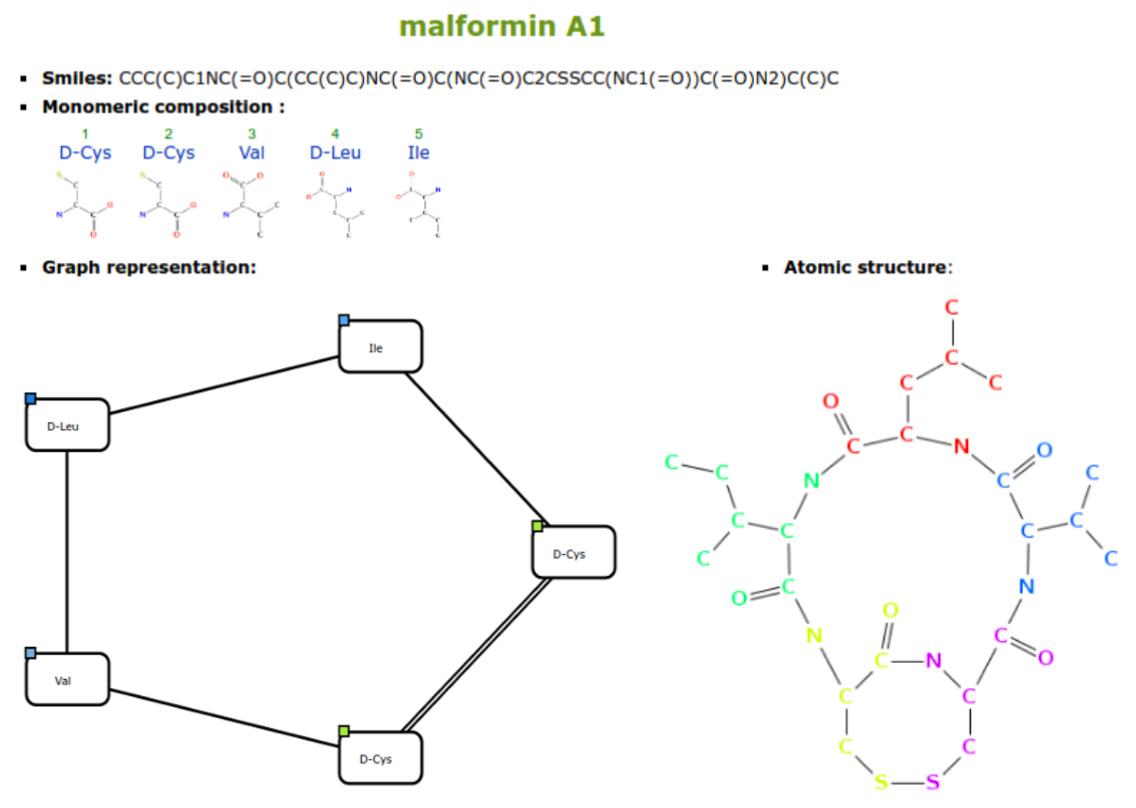
\includegraphics[width=400px]{figs/malformin_A1.png}
     % On the other hand, you must use eps files
     % \includegraphics[height=4cm,width=6cm]{figs/fig1.eps}
   \end{center}
   \caption{Structure representations of the malformin A1 in the Norine database.}
   \label{fig:malformin}
 \end{figure}


The Norine database is the reference NRP knowledge base, containing more than 1500 peptides composed of almost 600 different monomers (different building blocks including amino acids).
In the database, each NRP referenced have a dedicated web page with a lot of informations about their provenance, their composition and their pharmaceutical activities.
The most important information are their monomeric structure/composition (see figure \ref{fig:malformin}, on the left).
The monomeric representation, that we also called the biological structure, correspond to the nearest representation of the NRP assembly process.
In this representation, each node correspond to a molecule that had been included in the NRP during the synthesis.
The other representation (\ref{fig:malformin}, on the right), is the atomic representation, obtained by reconstruction after a mass spectrum analysis.
The knowledge of the monomeric representation is the most important information about a peptide because it is needed to fully understand the synthesis pathway.
It also as been proved[TODO] that, int he majority of the cases, the pharmaceutical activity can be infer from this only one information.

Since 2016, the Norine database is open to the crowdsourcing.
External users can submit new peptides to improve the data quantity of the database.
A complete procedure of submission and reviewing had been set up to guaranty the quality of these data.
Nevertheless, we know that many NRP discovered are not present in the Norine database and this process is not allowing a massive addition of data.
This is also not allowing the correction of wrong data that add been entered before the set up.

In the next parts of this article we will have a quick overview of the current work on data curation and database filling.


\section{Improving the data quality}

In the Bonsai group, we developed a tool to create automatic annotations of NRP called smiles2monomers (s2m).
From a SMILES (a textual atomic representation of a molecule[TODO]), s2m infer the monomeric structure of the NRP.
On one side, as we said during the introduction, the most useful information is the monomeric structure of NRP.
On the other side, almost every NRP are characterised by mass spectrum experiments, so we often only know their atomic structure.
So, s2m is a very powerful tool for the NRP community.

 \begin{figure}
   \begin{center}
     % if you have pdflatex installed, you can use pdf files as graphics
     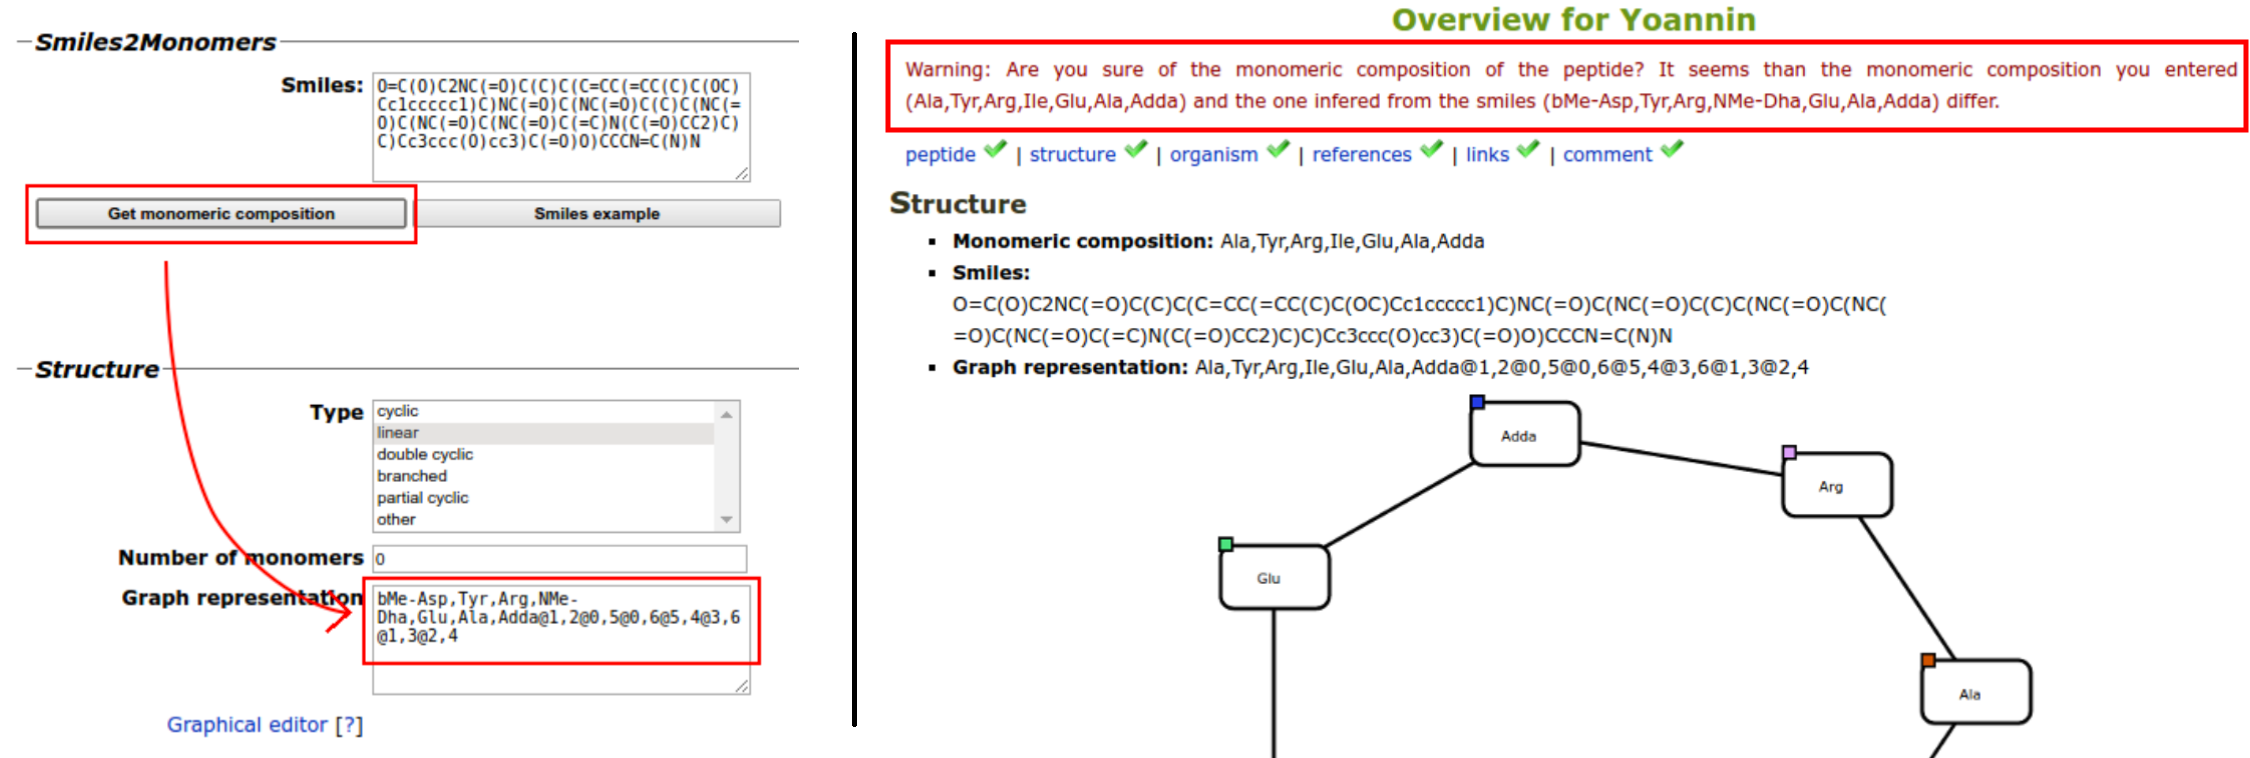
\includegraphics[width=400px]{figs/warnings.png}
     % On the other hand, you must use eps files
     % \includegraphics[height=4cm,width=6cm]{figs/fig1.eps}
   \end{center}
   \caption{Quality controls in the MyNorine software.}
   \label{fig:warnings}
 \end{figure}

In the Norine database, a significative amount of NRP entries (~30\%) are filled with both of the atomic and monomeric structures.
We used s2m on the atomic structures to verify the integrity of the data and we found a few errors (~50 with a wrong atomic or monomeric structure).
To avoid the insertion of new errors, we included the s2m software in the crowdsourcing tool MyNorine.
When a user want to add a new compound s2m is used during two validation steps.
First, when the user fill the SMILES area, myNorine can automatically create the monomeric structure (see figure \ref{fig:warnings}, on the left).
Secondly, if the user did not explicitly generate the monomeric structure, s2m run in background to compare the result with the manually entered structure.
If the automatic and manual annotations are not equivalent, the MyNorine tool will raise a warning to the user (see figure \ref{fig:warnings}, on the right)

\section{Improving the data quantity}

\section{Conclusion and perspectives}



 \bibliography{jobim_proceedings}
 
\end{document}

